\chapter{Strains}
\label{chap:strains}

\section*{Chapter description}

In this chapter, numerical results from strain calculations are presented along with the analysis.
Beginning from elastic characteristics of investigated materials, e.g. lattice constants, space groups, elastic constants, moving to electronic properties.
Band structures, orbital compositions, effective masses, and deformation potentials were calculated and described in detail.
The discussion and most important conclusions are also underlined.
All calculations provided here were performed with the ABINIT\cite{abinit1,abinit2,libxc} software package at the Wrocław Centre of Networking and Supercomputing.
\ornament
\section{Elastic properties}

As it was mentioned in chapter \ref{chap:theory} different pseudopotentials and exchange--correlation functionals are available to choose from.
Each of them will perform better depending on the type of material and properties that are of particular interest.
Group IV materials have already been heavily investigated, also in case of technical details in \abinitio\ calculations.
From the report \cite{LDA_choice} it is clear that, for realistic structural properties, \LDA\ functional is the most suitable for the four chosen materials.
The \PAW\cite{paw, paw2} pseudopotential is taken as complementary to \LDA, due to resulting realistic forces.
In case of electronic structure calculations, the most prominent choice is \mBJLDA\cite{mBJLDA, mBJLDA2}, which allows the user to obtain accurate band gaps.
Unfortunately, ABINIT lacks support for \PAW\ usage along with \mBJLDA, so instead the \HGH\cite{hgh} pseudopotential was used.

We begin the discussion of the results from structural and elastic properties of investigated structures, at equilibrium and at applied strains.
Table \ref{Tab:strain_lattice} shows the experimental and calculated lattice constants (in this work and from the literature).
An excellent agreement of the calculated values with the experimental ones confirms the appropriate choice of the exchange-correlation functional and the \PAW\ data, which also enhances the credibility of other results.

\begin{table}[!htbp]
    \caption{Lattice constants (\AA).}
    \centering
    \begin{tabular}{|c|c|c|c|}
    \hline
    material & this work & \LDA\ reference \cite{LDA_choice} & exp. \cite{LDA_choice} \\ \hline
    C  & 3.530     & 3.536     & 3.544   \\ \hline
    Si & 5.402     & 5.407     & 5.415   \\ \hline
    Ge & 5.627     & 5.632     & 5.639   \\ \hline
    Sn & 6.471     & 6.481     & 6.474 \\  \hline                      
    \end{tabular}
    \label{Tab:strain_lattice}
\end{table}

As mentioned previously, the strains are applied with respect to $[100]$, $[110]$, and $[111]$ directions, axial (along the directions) and biaxial (in the planes perpendicular to the directions).
In Fig. \ref{Fig:strain_scheme} the strains are shown schematically together with the relations between the relative changes in a linear dimension: optimized ($\epsopt$) and the corresponding induced change ($\epsind$).

\begin{figure}[!htbp]
	\centering
	\includegraphics[width=0.9\textwidth]{/strain/strain_scheme.pdf}
	\caption{Relative changes in linear dimensions, optimized ($\epsopt$) vs.induced  ($\epsind$), for axial strains (left panels) and biaxial strains (right panels).}
	\label{Fig:strain_scheme}
\end{figure}

As explained in the previous chapter, in the case of $[110]$ direction and for the axial strain only the maximum value of the $\epsopt$ is shown, i.e. for the $[100]$ direction.
The corresponding Poisson's ratios are listed in Tab. \ref{Tab:strain_Poisson}.

\begin{table}[!htbp]
    \caption{Poisson's ratios ($\poisson$) for axial (type 1) and biaxial (type 2) strains.}
    \centering
    \begin{tabular}{|c|c|c|c|c|c|c|c|}
        \hline
        \multirow{2}{*}{\begin{tabular}[c]{@{}c@{}}material\end{tabular}} & \multicolumn{2}{c|}{100} & \multicolumn{3}{c|}{110}        & \multicolumn{2}{c|}{111} \\ \cline{2-8} 
        & 1           & 2          & \multicolumn{2}{c|}{1} & 2      & 1           & 2          \\ \hline
        C                                                                      & 0.12        & 0.27       & 0.13       & 0.01      & 0.15   & 0.05        & 0.11       \\ \hline
        Si                                                                     & 0.29        & 0.81       & 0.38       & 0.07      & 0.55   & 0.19        & 0.46       \\ \hline
        Ge                                                                     & 0.29        & 0.77       & 0.38       & 0.03      & 0.48   & 0.17        & 0.40       \\ \hline
        Sn                                                                     & 0.34        & 1.00       & 0.49       & 0.04      & 0.66   & 0.22        & 0.57       \\ \hline
    \end{tabular}
    \label{Tab:strain_Poisson}
\end{table}

Some interesting features of the optimized structures can be observed:
\begin{enumerate}
    \item the relaxation under axial strain is in all the cases significantly smaller than under biaxial strain, with the biggest difference in Sn $[100]$ ($0.34$ vs $1.00$),
    \item generally the Poisson's ratios increase from C to Sn, except for Si and Ge where in most cases a sudden drop in the values is observed,
    \item the highest value of $\poisson=1$ is for Sn $[100]$ biaxial (which means that the free lattice parameter changes as much as the fixed one),
    \item the smallest one $\poisson=0.01$ for C $[110]$ axial (which means that the free lattice parameter almost does not change when the fixed one is varied.
\end{enumerate}
Thus the $\poisson$ varies in a large range of values (from $0.01$ to $1.00$) and no systematic behavior can be found (except for features mentioned above).

The strains lead to symmetry breaking which is characterized in Tab. \ref{Tab:strain_space}.
In the table one can find the numbers of space groups of equilibrium and strained diamond-like lattices, as well as the names and multiplicity of chosen high symmetry points in the \BZ.
As it can be seen, in six cases the star--degenerate energies in equilibrium $X$ and $L$ points split into two classes, which is also reflected in the energy gaps graphs which may behave quite differently for split points.

\begin{table}[!htbp]
    \caption{Space groups changes of characteristic \BZ\ points in strained diamond type lattice (numbers in parentheses denote the multiplicity of a given point).}
    \centering
    \begin{tabular}{|c|c|c|c|c|}
    \hline
         & equil.          & 100                  & 110                 & 111                  \\ \hline
        \multirow{2}{*}{\begin{tabular}[c]{@{}l@{}}space\\ group \#\end{tabular}} & \multirow{2}{*}{227} & \multirow{2}{*}{141} & \multirow{2}{*}{74} & \multirow{2}{*}{166} \\
         &                      &                      &                     &                      \\ \hline
        \multirow{3}{*}{\begin{tabular}[c]{@{}l@{}}special\\ points\end{tabular}} & $\Gamma$             & $\Gamma$             & $\Gamma$            & $\Gamma$             \\ \cline{2-5} 
         & X(6)                 & X(4)/M(2)            & X(2)/R(4)           & FB(6)                \\ \cline{2-5} 
         & L(8)                 & N(8)                 & T(4)/S(4)           & L(6)/T(2)            \\ \hline
    \end{tabular}
    \label{Tab:strain_space}
\end{table}

To provide a better comprehension of the changes in \BZ\ on Fig. \ref{Fig:strain_BZ} can be found visualizations of each occurring space group \BZ's.

\begin{figure*}[!htbp]
    \centering
    \begin{subfigure}[b]{0.475\textwidth}
        \centering
        \includegraphics[width=1.\textwidth]{/strain/216.pdf}
        \caption{$\#227$ -- isotropic strains}
        \label{Fig:strain_227}
    \end{subfigure}
    \hfill
    \begin{subfigure}[b]{0.475\textwidth}  
        \centering 
        \includegraphics[width=1.\textwidth]{/strain/141.pdf}
        \caption{$\#141$ -- $[100]$ straining direction}
        \label{Fig:strain_141}
    \end{subfigure}
    \vskip\baselineskip
    \begin{subfigure}[b]{0.475\textwidth}   
        \centering 
        \includegraphics[width=1.\textwidth]{/strain/74.pdf}
        \caption{$\#74$ -- $[110]$ straining direction}  
        \label{Fig:strain_74}
    \end{subfigure}
    \hfill
    \begin{subfigure}[b]{0.475\textwidth}   
        \centering 
        \includegraphics[width=1.\textwidth]{/strain/166.pdf}
        \caption{$\#166$ -- $[111]$ straining direction}  
        \label{Fig:strain_166}
    \end{subfigure}
    \caption{Visualization of \BZ\ taken from Bilbao Crystallographic Server}
    \label{Fig:strain_BZ}
\end{figure*}

The applied strain, on the one hand, leads to relaxation of free degrees of freedom but on the other it induces stress, as a response of the system.
For axial strain for a given axis the stress appears on the plain perpendicular to the axis, whereas for biaxial strain the stress appears on the plains parallel to the axis.
The axial symmetry exists except for $[110]$ direction and biaxial uniform strain, in which case there is a maximum value of the stress (at $(100)$ plane) and minimum one (at $(110)$ plane).
The relationship between stress and strain is represented by the first (C1) and the second order (C2) elastic constants in the quadratic function approximation.
The elastic constants described above are presented in Tab. \ref{Tab:strain_pressure}.
Here, the chemical trend is clear: the bigger is the atomic number of the element the smaller the elastic constant.
The biggest value of the linear constant C1 is for C at isotropic strain ($14.4$ $GPa$), and the smallest one for Sn $[100]$ axial strains ($0.45$ $GPa$).
As for the second order coefficients, which account for the bowing of the stress vs strain curve, the biggest value is again for C isotropically strained (-0.85 $GPa$) and the smallest one for Sn biaxially strained with respect to $[110]$ axis ($-0.0014$ $GPa$).
The negative values of C2 correspond to concave behavior.
It is easy to note that at considered strains the resulted strain do not exceed $100 GPa$ (in diamond) and a few $GPa$ in Sn.

\begin{table}[!htbp]
    \caption{First (C1) and second order (C2) elastic constants defined in this work ($GPa$).}
    \centering
    \begin{tabular}{|c|c|c|c|c|c|c|c|c|c|}
        \hline
         & fit parameter & 100 biaxial & 100 axial & \multicolumn{2}{c|}{110 biaxial} & 110 axial & 111 biaxial & 111 axial & isotropic \\ \hline
        \multirow{2}{*}{C}  & C1   & 1230  & 1070 & 1240 & 1380 & 1210 & 1340 & 1250 & 1440 \\ \cline{2-10} 
         &  C2   & -4480 & -624 & -3910 & -6410 & -3670  & -6020 & -3730 & -8480   \\ \hline
        \multirow{2}{*}{Si} &  C1   & 175  & 124  & 185  & 227 & 162 &  223  & 180  & 298    \\ \cline{2-10} 
         & C2   & -595 & -224  & -99 & -444 & -385 & -722 & -88 & -2050   \\ \hline
        \multirow{2}{*}{Ge} &  C1   & 133  & 93.9  & 142  & 180 & 128 &  172  & 143  & 223    \\ \cline{2-10} 
         & C2   & -610  & -205  & -145 & -538 & -362 & -884 & -19 & -1680   \\ \hline
        \multirow{2}{*}{Sn} &  C1   & 68.3  & 44.6  & 76.4 & 101 & 64.9  & 96.6   & 74.3  & 141    \\ \cline{2-10} 
         & C2   & -292 & -143  & -26  & -1880 & -116 & -442 & -81  & -1100     \\ \hline
    \end{tabular}
    \label{Tab:strain_pressure}
\end{table}

For verification purposes, the standard elastic constants (for linear regime) have been evaluated from our $C1$ and $C2$ constants.
The results are presented in Tab. \ref{Tab:strain_elastic} and show satisfactory agreement with the textbook data\cite{nsm}.

\begin{table}[!htbp]
    \caption{Standard elastic constants (GPa) evaluated from data presented in Tab. \ref{Tab:strain_pressure} and their comparison with the textbook values\cite{nsm}.}
    \centering
    \begin{tabular}{|c|c|c|c|c|}
        \hline
        & C             & Si           & Ge           & Sn          \\ \hline
        calc. $c_{11}$  & 1100 $\pm 50$ & 160 $\pm 20$ & 120 $\pm 25$ & 66 $\pm 9$  \\ \hline
        exp. $c_{11}$  & 1079          & 166          & 126          & 73.3        \\ \hline
        calc. $c_{12}$ & 160 $\pm 30$  & 70 $\pm 6$   & 52 $\pm 7$   & 50 $\pm 4$  \\ \hline
        exp. $c_{12}$  & 124           & 64           & 44           & 67.7        \\ \hline
        calc. $c_{44}$ & 490 $\pm 40$  & 62 $\pm 8$   & 59 $\pm 4$   & 23 $\pm 10$ \\ \hline
        exp. $c_{44}$  & 578           & 79.6         & 67.7         & 2.19        \\ \hline
    \end{tabular}
    \label{Tab:strain_elastic}
\end{table}
\ornament

\section{Band structures}

The evolution of the electronic band structures with applied strains have been represented by changes in the energy differences between the \VB\ maxima and and \CB\ minima at $\Gamma$ point (direct band gaps) and between the \VB\ maxima and conduction band minima along high symmetry directions $\Delta$ and  $\Lambda$ (indirect band gaps).
This choice is justified by the fact that the density of states extrema are present at these points and the direct and indirect optical transitions, observed in various spectroscopy experiment take place.
The rule of the band gaps presentation, for Ge isotropically strained, is shown in Fig. \ref{Fig:strain_gap-example}.
For completeness we also present the evolution of the \LH--\HH\ band splitting (Tab. \ref{Tab:strain_split}).

\begin{table}[!htbp]
    \centering
    \caption{Linear coefficients \LH--\HH\ bands splitting as function of strain (eV/\%).}
    \begin{tabular}{|c|c|c|c|c|}
        \hline
        strain & C     & Si    & Ge & Sn \\ \hline
        100 biaxial      & -0.22 & -0.14 & -0.11 & -0.09 \\ \hline
        100 axial     & 0.19  & 0.09  & 0.08 & 0.06 \\ \hline
        110 biaxial      & 0.11  & 0.11  & 0.06 & 0.06 \\ \hline
        110 axial     & -0.10  & -0.11 & -0.06 & -0.06 \\ \hline
        111 biaxial      & -0.04 & -0.11 & -0.04 & -0.05 \\ \hline
        111 axial     & 0.02  & 0.07  & 0.05 & 0.04 \\ \hline
    \end{tabular}
    \label{Tab:strain_split}
\end{table}

\begin{figure}[!htbp]
    \centering
    \includegraphics[width=0.7\textwidth]{/strain/gaps_example.pdf}
    \caption{Pictorial diagram of the band gaps presentation, on the example of isotropically strained Ge. a) shows how band gaps change with strain, while b), c) and d) visualize band structures under given stains.}
    \label{Fig:strain_gap-example}
\end{figure}

The analysis begins from the discussion of typical qualitative behavior of bands which is shown in Fig. \ref{Fig:strain_fatband_scheme}.
The orbital character visualization has been used, i.e. the dots of varying color represent a contribution of atomic orbitals to a wave function corresponding to a particular point on the energy diagram (for details see the figure caption), i.e. the color stands for the kind of atomic orbital (spherical harmonics, $s,p,d,...$) and the intensity, the relative contribution.
Two cases are presented there: isotropically strained Sn, whose behavior is similar to that of Ge, and biaxially strained Si with respect to $[100]$ axis, which represents behavior of diamond-like lattices under non--isotropic strains.

\begin{figure}[!htbp]
    \centering
    \includegraphics[width=1\textwidth]{/strain/fatband_scheme.pdf}
    \caption{Typical qualitative features of bands behavior as a function of strain for diamond-like group IV crystals, on the example of isotropically strained Sn in a) $-6\%$  b) $-4\%$ and c) $-1\%$ , and biaxially strained Si with respect to [100] direction Si in d) $-4\%$, e) $0\%$ (equilibrium structure) and f) $4\%$. "Fat bands" representation is used, i.e. the color stands for the kind of orbital and the intensity for the relative contribution; here green colour denotes $p$ atomic orbital and red - $s$ orbital; here, the values of gaps are not correct, because of the known deficiency of \DFT\ (the band gap problem).}
    \label{Fig:strain_fatband_scheme}
\end{figure}

In the first case (Fig. \ref{Fig:strain_fatband_scheme} a,b,c) three situations can be distinguished:
\begin{enumerate}
    \item[a)] at a range of strain represented here by $-6\%$ compressive strain, the open direct band gap exists, with $\Gamma_7^-$ (irreducible representation) \CB\ minimum, degenerate \VBM\ $\Gamma_8^+$ and \SO\ split-off band $\Gamma_7^+$,
    \item[b)] at a range of strain represented here by $-4\%$ compressive strain the direct gap is closed, Sn becomes semi--metallic, and the $\Gamma_7^-$ point goes below the degenerate $\Gamma_8^+$ (negative direct band gap),
    \item[c)] at a range of strain represented here by $-1\%$ compressive strain, $\Gamma_7^-$ goes below the split-off band $\Gamma_7^+$.
\end{enumerate}

In the case b) and c) it may happen that certain region of \CB\ goes below the Fermi level and then Sn becomes a metal.
Similar situation can be observed in Ge (although at different ranges of strain), as well as in GeSn alloy, at specific composition/strain ranges \cite{Polak.2017}.
In the second case (Fig. \ref{Fig:strain_fatband_scheme} d,e,f) also the three typical situations appear:
\begin{enumerate}
    \item[d)] at a range of strains (biaxial, with respect to $[100]$), represented here by $-4\%$ compressive strain, the degeneracy of \HH\ and \LH\ bands is removed (due symmetry break) and inversion of \HH\ and \LH\ bands appears,
    \item[e)] at equilibrium lattice constant, there is a quite big direct band gap (about $2.3$ eV), degenerate at $\Gamma$ \HH\ and light hole \LH\ bands, and slightly detached \SO\ split-off band; in this case Si (and also C) the isotropic strain results only in the vertical movement of bands and no inversion is observed,
    \item[f)] at a range of strains, represented here by $+4\%$ tensile strain, the degeneracy of \HH\ and \LH\ bands is removed but no band inversion takes place.
\end{enumerate}

It should be stressed out that the values of the band gaps given above were calculated with \LDA\ functional, and therefore are not correct.
They are here only for schematic representation of the behavior of the bands and their symmetries under strain.
The expected correct values are given in Fig. \ref{Fig:strain_ge_gaps} and Tabs. \cref{Tab:strain_gap_iso,Tab:strain_gap_uni_compressive,Tab:strain_gap_uni_tensile,Tab:strain_gap_bi_compressive,Tab:strain_gap_bi_tensile}, where the \mBJLDA\ functional has been used.

\begin{figure}[!htbp]
    \centering
    \includegraphics[width=0.6\textwidth]{/strain/C-gaps.pdf}
    \caption{Band gaps in C diamond-like crystal. Bottom-left graph -- isotropic strain; Above -- left column: biaxial strain, right column: axial strain. From the first to the last row, respectively: strains with respect to directions ${[100]}$, ${[110]}$, ${[111]}$. Purple line is the difference between light and heavy hole bands, green lines are direct band gaps, red and orange are indirect band gaps ($\Gamma$-X), blue are indirect band gaps ($\Gamma$-L). Dashed lines are with respect to the top of the heavy hole band, continuous to the top of the light hole band.}
    \label{Fig:strain_c_gaps}
\end{figure}

\begin{figure}[!htbp]
    \centering
    \includegraphics[width=0.6\textwidth]{/strain/Si-gaps.pdf}
    \caption{Band gaps in Si diamond-like crystal. Bottom-left graph -- isotropic strain; Above -- left column: biaxial strain, right column: axial strain. From the first to the last row, respectively: strains with respect to directions ${[100]}$, ${[110]}$, ${[111]}$. Purple line is the difference between light and heavy hole bands, green lines are direct band gaps, red and orange are indirect band gaps ($\Gamma$-X), blue are indirect band gaps ($\Gamma$-L). Dashed lines are with respect to the top of the heavy hole band, continuous to the top of the light hole band.}
    \label{Fig:strain_si_gaps}
\end{figure}

\begin{figure}[!htbp]
    \centering
    \includegraphics[width=0.6\textwidth]{/strain/Ge-gaps.pdf}
    \caption{Band gaps in Ge diamond-like crystal. Bottom-left graph -- isotropic strain; Above -- left column: biaxial strain, right column: axial strain. From the first to the last row, respectively: strains with respect to directions ${[100]}$, ${[110]}$, ${[111]}$. Purple line is the difference between light and heavy hole bands, green lines are direct band gaps, red and orange are indirect band gaps ($\Gamma$-X), blue are indirect band gaps ($\Gamma$-L). Dashed lines are with respect to the top of the heavy hole band, continuous to the top of the light hole band.}
    \label{Fig:strain_ge_gaps}
\end{figure}

\begin{figure}[!htbp]
    \centering
    \includegraphics[width=0.6\textwidth]{/strain/Sn-gaps.pdf}
    \caption{Band gaps in Sn diamond-like crystal. Bottom-left graph -- isotropic strain; Above -- left column: biaxial strain, right column: axial strain. From the first to the last row, respectively: strains with respect to directions ${[100]}$, ${[110]}$, ${[111]}$. Purple line is the difference between light and heavy hole bands, green lines are direct band gaps, red and orange are indirect band gaps ($\Gamma$-X), blue are indirect band gaps ($\Gamma$-L). Dashed lines are with respect to the top of the heavy hole band, continuous to the top of the light hole band.}
    \label{Fig:strain_sn_gaps}
\end{figure}

The defined above gaps as functions of strain, for all systems and all applied strains are presented in Fig. \ref{Fig:strain_ge_gaps} and Tabs. \cref{Tab:strain_gap_iso,Tab:strain_gap_uni_compressive,Tab:strain_gap_uni_tensile,Tab:strain_gap_bi_compressive,Tab:strain_gap_bi_tensile}, whose meaning is explained in Fig. \ref{Fig:strain_gap-example}.
A striking feature of almost all the plots (except for isotropic case) is a sharp change in the value of the linear coefficient between the tensile and the compressive strain (even its sign) at the zero strain point.
As it has been already explained the reason for such behavior is the inversion of \HH\ and \LH\ bands, as demonstrated in Fig. \ref{Fig:strain_fatband_scheme} (d,e,f).
This is due to the opposite direction of movements of \HH\ and \LH\ bands at applied compressive and tensile strains (see Tab. \ref{Tab:strain_split}).
The only situation at which this not happens is the isotropic strain, and here the change of gaps is monotonic in the full range of strain.
Various behavior of bands in directions from $\Gamma$ to X and L star points ($\Delta$ and $\Lambda$ lines, respectively) has been observed due to strain induced symmetry breaking, which is a known feature, and the appropriate distinction is made in Tabs. \cref{Tab:strain_gap_iso,Tab:strain_gap_uni_compressive,Tab:strain_gap_uni_tensile,Tab:strain_gap_bi_compressive,Tab:strain_gap_bi_tensile}.
Another rather obvious feature is  that the plots for tensile and compressive strains are qualitatively similar except they are "reflected" with respect to zero-strain vertical line.
This is because applying the biaxial/axial compressive strain leads to the qualitative change in the structure the same as under the axial/biaxial tensile strain.
The changes in the structures under biaxial strains are more pronounced than under axial ones, because the Poisson ratios are higher, and that is why the changes in the gaps are bigger.
Another distinct feature is that in most cases the changes in the gaps are almost linear.
There are, however, some exceptions, like direct band gaps in Ge at $[110]$ and $[111]$ case where big bowings at compressive strains can be seen.
From applications point of view the most interesting are the cases where indirect--direct gap transition induced by strain appears, which in the case of Ge takes place in almost all biaxial strains (except $[111]$) as well as at isotropic strain.
Also in Sn at uniform compressive strain a direct open gap appear.
It should  be mentioned that strain is often applied jointly with mixing of elements (alloying) (see e.g. \cite{Polak.2017}), which opens large opportunities of band structure formations towards wanted in particular applications features.

\begin{table}[!htbp]
    \centering
    \caption{Equilibrium band gaps (eV) and the linear coefficients of gap changes (eV/\%) for isotropic strains.}
    \begin{tabular}{|c|c|c|c|c|}
        \hline
        \multicolumn{2}{|c|}{}      & $\Gamma-\Gamma$ & $\Gamma-X$ & $\Gamma-L$ \\ \hline
        \multirow{2}{*}{C}  & gap    & 7.38            & 5.53       & 8.79       \\ \cline{2-5} 
                            & lin. coef.  & -0.08           & -0.04      & -0.12      \\ \hline
        \multirow{2}{*}{Si} & gap    & 3.20            & 1.32       & 2.34       \\ \cline{2-5} 
                            & lin. coef.  & -0.02           & 0.06       & -0.10      \\ \hline
        \multirow{2}{*}{Ge} & gap    & 0.89            & 0.94       & 0.74       \\ \cline{2-5} 
                            & lin. coef.  & -0.30           & 0.04       & -0.11      \\ \hline
        \multirow{2}{*}{Sn} & gap    & -0.31           & 0.66       & 0.11       \\ \cline{2-5} 
                            & lin. coef.  & -0.23           & 0.03       & -0.08      \\ \hline
    \end{tabular}
    \label{Tab:strain_gap_iso}
\end{table}

\begin{table}[!htbp]
    \centering
    \caption{Linear coefficients of band gap changes for axial compressive strains (eV/\%).}
    \begin{tabular}{|c|c|c|c|c|}
        \hline
        gap          & C & Si & Ge & Sn \\ \hline
        $\Gamma-\Gamma\,[100]$ & 0.20  & 0.08  & 0.02  & -0.07 \\ \hline
        $\Gamma-X\,[100]$ & 0.02 & 0.03  & 0.02 & -0.06 \\ \hline
        $\Gamma-M\,[100]$ & 0.31 & 0.15  & 0.14 & 0.04 \\ \hline
        $\Gamma-N\,[100]$ & 0.21 &  0.07  & 0.06 & -0.03 \\ \hline
        $\Gamma-\Gamma\,[110]$ & 0.26 & 0.14 & 0.01 & -0.06 \\ \hline
        $\Gamma-X\,[110]$  & 0.02  & 0.07 & 0.03 & -0.04 \\ \hline
        $\Gamma-R\,[110]$  & 0.10 & 0.10 & 0.08 & 0.01 \\ \hline
        $\Gamma-T\,[110]$  & 0.24 & 0.10 & 0.08 & 0.01 \\ \hline
        $\Gamma-S\,[110]$  & 0.26 & 0.02 & -0.01 & -0.07 \\ \hline
        $\Gamma-\Gamma\,[111]$  & 0.09 & 0.09 & 0.003 & -0.04 \\ \hline
        $\Gamma-FB\,[111]$ & 0.02 & 0.08 & 0.05 & 0.002 \\ \hline
        $\Gamma-L\,[111]$  & 0.09 & -0.01 & -0.03 & -0.06 \\ \hline
        $\Gamma-T\,[111]$  & 0.02 & 0.15 & 0.13 & 0.07 \\ \hline
    \end{tabular}
    \label{Tab:strain_gap_uni_compressive}
\end{table}

\begin{table}[!htbp]
    \centering
    \caption{Linear coefficients of band gap changes for axial tensile strains (eV/\%).}
    \begin{tabular}{|c|c|c|c|c|}
        \hline
        gap          & C & Si & Ge & Sn \\ \hline
        $\Gamma-\Gamma\,[100]$  & -0.13  & -0.05 & -0.09 & 0.05 \\ \hline
        $\Gamma-X\,[100]$  & -0.16  & -0.06  & -0.07 & -0.011 \\ \hline
        $\Gamma-M\,[100]$  & 0.09  & 0.05 & 0.05 & 0.09 \\ \hline
        $\Gamma-N\,[100]$  & -0.17  & -0.08  & -0.06 & -0.0008 \\ \hline
        $\Gamma-\Gamma\,[110]$  & -0.16 & -0.09 & -0.11 & 0.04 \\ \hline
        $\Gamma-X\,[110]$  & -0.22 & -0.1 & -0.09 & -0.04 \\ \hline
        $\Gamma-R\,[110]$  & 0.02 & -0.002 & 0.002 & 0.05 \\ \hline
        $\Gamma-T\,[110]$  & -0.10 & -0.005 & -0.006 & 0.04 \\ \hline
        $\Gamma-S\,[110]$  & -0.10 & -0.13 & -0.11 & -0.04 \\ \hline
        $\Gamma-\Gamma\,[111]$  & -0.25 & -0.16 & -0.12 & 0.03 \\ \hline
        $\Gamma-FB\,[111]$ & -0.03 & -0.03 & -0.02 & 0.01 \\ \hline
        $\Gamma-L\,[111]$  & -0.24 & -0.09 & -0.08 & -0.03 \\ \hline
        $\Gamma-T\,[111]$  & 0.02 & 0.07 & 0.06 & 0.09 \\ \hline
    \end{tabular}
    \label{Tab:strain_gap_uni_tensile}
\end{table}

\begin{table}[!htbp]
    \centering
    \caption{Linear coefficients of band gap changes for biaxial compressive strains (eV/\%).}
    \begin{tabular}{|c|c|c|c|c|}
        \hline
        gap          & C & Si & Ge & Sn \\ \hline
        $\Gamma-\Gamma\,[100]$  & 0.09  & 0.06  & -0.07 & -0.06 \\ \hline
        $\Gamma-X\,[100]$  & 0.17  & 0.13 & 0.13 & 0.05 \\ \hline
        $\Gamma-M\,[100]$  & -0.16 & -0.03 & -0.06 & -0.1 \\ \hline
        $\Gamma-N\,[100]$  & 0.10  & 0.08 & 0.04 & -0.01 \\ \hline
        $\Gamma-\Gamma\,[110]$  & 0.16 & 0.12 & -0.05 & -0.05 \\ \hline
        $\Gamma-X\,[110]$  & 0.22 & 0.19 & 0.16 & 0.10 \\ \hline
        $\Gamma-R\,[110]$  & 0.02 & 0.04 & 0.02 & -0.03 \\ \hline
        $\Gamma-T\,[110]$  & 0.10 & -0.10 & -0.11 & -0.13 \\ \hline
        $\Gamma-S\,[110]$  & 0.10 & 0.11 & 0.08 & 0.04 \\ \hline
        $\Gamma-\Gamma\,[111]$  & 0.23 & 0.21 & -0.04 & -0.05 \\ \hline
        $\Gamma-FB\,[111]$ & 0.02 & 0.11 & 0.08 & 0.02 \\ \hline
        $\Gamma-L\,[111]$  & 0.16 & 0.05 & 0.03 & -0.001 \\ \hline
        $\Gamma-T\,[111]$  & -0.12 & -0.16 & -0.18 & -0.20 \\ \hline
    \end{tabular}
    \label{Tab:strain_gap_bi_compressive}
\end{table}

\begin{table}[!htbp]
    \centering
    \caption{Linear coefficients of band gap changes for biaxial tensile strains (eV/\%).}
    \begin{tabular}{|c|c|c|c|c|}
        \hline
        gap          & C & Si & Ge & Sn \\ \hline
        $\Gamma-\Gamma\,[100]$  & -0.27  & -0.13 & -0.20 & 0.10 \\ \hline
        $\Gamma-X\,[100]$  & -0.06  & -0.01 & -0.005 & 0.10 \\ \hline
        $\Gamma-M\,[100]$  & -0.35  & -0.17 & -0.17 & -0.05 \\ \hline
        $\Gamma-N\,[100]$  & -0.33 & -0.16 & -0.14 & -0.002 \\ \hline
        $\Gamma-\Gamma\,[110]$  & -0.26 & -0.16 & -0.22 & 0.06 \\ \hline
        $\Gamma-X\,[110]$  & -0.02 & -0.05 & -0.03 & 0.03 \\ \hline
        $\Gamma-R\,[110]$  & -0.10 & -0.05 & -0.04 & 0.02 \\ \hline
        $\Gamma-T\,[110]$  & -0.24 & -0.18 & -0.15 & -0.06 \\ \hline
        $\Gamma-S\,[110]$  & -0.26 & -0.07 & -0.05 & 0.03 \\ \hline
        $\Gamma-\Gamma\,[111]$  & -0.15 & -0.10 & -0.21 & 0.03 \\ \hline
        $\Gamma-FB\,[111]$ & -0.05 & -0.03 & -0.02 & 0.01 \\ \hline
        $\Gamma-L\,[111]$  & -0.18 & -0.05 & -0.04 & 0.01 \\ \hline
        $\Gamma-T\,[111]$  & -0.12 & -0.22 & -0.20 & -0.12 \\ \hline
    \end{tabular}
    \label{Tab:strain_gap_bi_tensile}
\end{table}

Both band structures and orbital compositions were calculated for all considered systems.
Although not shown here, the database of this results is kept, and can be shared on request.

A good verification of presented here results is their comparison with available experimental data \cite{Ge-app2010, Ge-exp2011, Ge-exp2016, Ge-app2018}, presented in below (Fig.\ref{Fig:strain_exp}).
As it can be seen, for the \LH-\HH\ splitting the agreement is excellent. Also for direct gap in Ge the agreement is very good, taking into account the fact that the measurement was performed at room temperature, whereas the calculations correspond to zero temperature.
Considering about $10\%$ temperature induced reduction in the band gap  at $300K$ (tabular value) makes the agreement of obtained results with experiment very good.
Finally, the reported in \cite{Ge-exp2018} indirect-to-direct band gap crossing point at $1.94\%$ $[100]$ biaxial strain agrees very well with given prediction (see Fig. \ref{Fig:strain_ge_gaps}).
The presented below comparison strongly point at credibility of the provided computational results, since, the calculations are consistent regarding the methods applied.

\begin{figure}
    \centering
    \includegraphics[width=0.9\textwidth]{/strain/experiment_comparizon.pdf}
    \caption{Computational results vs. experimental data for germanium; upper left panel:  direct gap ${[100]}$ axial strain (according to \cite{Ge-exp2016}), upper right panel: ${[100]}$ biaxial \cite{Ge-exp2011} (the reductions of the experimental direct gaps are induced by temperature, $300K$), bottom panel: ${[100]}$ biaxial strain \LH-\HH \cite{Ge-app2018}, ${[100]}$ axial \LH-\HH \cite{Ge-app2010}.} 
    \label{Fig:strain_exp}
\end{figure}

\ornament

\section{Deformation potentials}

To have a complete image of the electronic band structure behaviour under strains, there were calculated the deformation potentials $a_v$, $a^{dir}$, $a^{ind}$, $b$, $d$, $\Xi_u^{\Delta}$, $\Xi_u^{L}$, as defined defined in \cite{pot-def}, i.e. the parameters describing the strain induced characteristic energies variation.
The results are gathered and compared with the literature data in Tab. \ref{Tab:strain_deformation}.
The main conclusion from the presented data is that the values of the relative deformation potentials (describing the changes in energy differences) agree well with the literature data, whereas the absolute ones (describing the changes in energies given with respect to the absolute energy reference point) differ significantly.
At this stage explanation of the variation in results remains unknown, however, in \cite{deformation-ref2} an experimental value of $a_v=-12.7$ eV for Ge, and in \cite{deformation-ref} a theoretical values for Ge of $a_v=-12.4$ eV  and for Si $a_v=-10.2$ eV are reported.
This means that there is quite a big discrepancy of data in the literature.
Nevertheless, in case of the results shown here there is precisely described procedure (in Sect. \ref{chap:methods}) to establish a frame for future discussion.

\begin{table}[!htbp]
\centering
\caption{Deformation potentials.}
\begin{tabular}{|c|c|c|c|c|}
\hline
                 & Si    & Si ref. & Ge    & Ge ref. \\ \hline
$\Delta_0$       & 0.05 & 0.04 \cite{pot-def}  & 0.29  & 0.30 \cite{pot-def}    \\ \hline
$a_v$            & -0.30$\pm$0.43  & 2.46 \cite{pot-def} & -4.0$\pm$0.55  & 1.24 \cite{pot-def}  \\ \hline
$b$              & -1.39$\pm$1.03 & -2.35 \cite{pot-def}    & -6.72$\pm$0.90 & -2.55 \cite{pot-def}  \\ \hline
$d$              & -0.37$\pm$1.01 & -5.32 \cite{pot-def}    & -10.00$\pm$3.19   & -5.50 \cite{pot-def}   \\ \hline
$a^{dir}$        & -0.65$\pm$0.02 & -0.48 \cite{pot-def}    & -9.59$\pm$0.42 & -9.48 \cite{pot-def}  \\ \hline
$a^{ind}$        & 1.74$\pm$0.05  & 1.72 \cite{pot-def} & -3.53$\pm$0.05 & -2.78 \cite{pot-def}  \\ \hline
$\Xi_u^\Delta$   & 8.80$\pm$0.09   & 8.70 \cite{pot-def}    & 9.50$\pm$0.10   & 9.02 \cite{mass-pot} \\ \hline
$\Xi_u^L$        & 14.30$\pm$0.04  & 13.85 \cite{mass-pot}  & 15.70$\pm$0.20  & 16.30 \cite{pot-def} \\ \hline
\end{tabular}
\label{Tab:strain_deformation}
\end{table}

\ornament

\section{Effective masses of charge carriers}

There are rather few results in the literature of the theoretical calculations of effective masses and, in particular, their dependencies on strains.
Some calculations using various methods, \abinitio, \TB, $\mathbf{k}\cdot \mathbf{p}$, are reported eg. in \cite{mass-dft, mass-tb, mass-kp}.
In this work a systematic first principles computational study has been performed of chosen effective masses dependence on strains, using the method described in chapter \ref{chap:methods}.
The results are presented in Figs. \cref{Fig:strain_mass_100,Fig:strain_mass_110,Fig:strain_mass_111,Fig:strain_mass_iso}.


\begin{table}[!htbp]
 \caption{Effective masses (in units of electron mass) in chosen \BZ\ points calculated in this work and compared with the literature reference data.}
 \centering
\begin{tabular}{|c|c|c|c|c|c|c|c|c|}
\hline
                    & $m_{eff}$ \textbackslash research & this work & GW \cite{mass-kp}     & EPM \cite{mass-kp}  & $\mathbf{k}\cdot \mathbf{p}$ \cite{mass-kp} & TB \cite{mass-tb}  & DFT \cite{mass-dft}  & exp.  \cite{mass-dft, mass-tb, mass-kp} \\ \hline
\multirow{6}{*}{Si} & $\Gamma$ (X dir.)         & 0.676    &        &       &              &       & 0.158 &       \\ \cline{2-9} 
                    & $\Gamma$ (L dir.)         & 0.514    &        &       &              &       &       &       \\ \cline{2-9} 
                    & X                         & 0.798    & 0.925  & 0.89  & 0.928        & 0.891 & 0.915 & 0.916 \\ \cline{2-9} 
                    & L                         & 1.92    & 1.8083 & 1.855 & 1.704        & 3.433 &       & 2.0     \\ \cline{2-9} 
                    & holes (X dir.)            & 0.327    &        &       &              & 0.276 & 0.22  & 0.275 \\ \cline{2-9} 
                    & holes (L dir.)            & 0.811    &        &       &              & 0.734 & 0.66  & 0.738 \\ \hline
\multirow{6}{*}{Ge} & $\Gamma$ (X dir.)         & 0.047    &        &       &              &       & 0.037 & 0.038 \\ \cline{2-9} 
                    & $\Gamma$ (L dir.)         & 0.05    &        &       &              &       &       &       \\ \cline{2-9} 
                    & X                         & 0.674    & 0.881  & 0.964 & 0.874        & 0.701 &       & 0.9   \\ \cline{2-9} 
                    & L                         & 1.69    & 1.626  & 1.763 & 1.59         & 1.584 & 1.66  & 1.58  \\ \cline{2-9} 
                    & holes (X dir.)            & 0.236    &        &       &              & 0.173 &   & 0.211 \\ \cline{2-9} 
                    & holes (L dir.)            & 0.602     &        &       &              & 0.531 &   & 0.502 \\ \hline
\end{tabular}
 \label{Tab:strain_masses}
\end{table}
Before the start of the discussion of the effect of strains on effective masses, there should be pointed out that provided data agree well with those reported in \cite{mass-dft, mass-tb, mass-kp} and experimental values referenced there (see Tab. \ref{Tab:strain_masses}).
This fact enhances the credibility of the discussion on the effect of strains.

First, note that in all the dependencies presented in Figs. \cref{Fig:strain_mass_100,Fig:strain_mass_110,Fig:strain_mass_111}, as expected, the qualitative behaviors for biaxial and axial strains are inverse with respect to zero strain, for the reason discussed previously.
One can distinguish a few characteristic cases of different qualitative behavior.
In the conduction band, for example, a very big increase in the Si effective mass  can be observed, at $\Gamma$ in $\Gamma$-$X$ direction, with $[100]$ axial tensile (or biaxial compressive) small ($1\%$) strain.
Such a behavior is connected with "flattening" of the band, and what is interesting, this does not happen in the $\Gamma$-$L$ direction.
A large increase can also be seen at $X$ under $[110]$ strains, both in Si and Ge, but at higher strains ($3-4\%$), and at $X$ under $[111]$ strains.
On the other hand, very small effective masses ($0.04$ at equilibrium) can be found in Ge at $\Gamma$, but an interesting fact is that at some strains ($[110]$ biaxial, $[111]$ biaxial, isotropic) the effective mass clearly tends to zero, which is connected with closing the direct gap, and results in high mobility of \CB\ electrons which has a practical meaning.
Apart from that there is a variety of cases where the change in the effective masses is regular but not very big (up to $100\%$, like at $[110]$ strains in Si) or looks almost constant but is irregular (like at $X$ $[100]$ strain, both in Si and Ge), which must be due to numerical noise (the results are extremely sensitive to any numerical uncertainties).
In the \VB\ the effective mass behavior is very spectacular because a described previously inversion of bands.
Thus, a sudden drop or increase of the effective mass is observed, depending on which band (\HH\ or \LH) is actually on the top.
The most spectacular change (by one order of magnitude) caused by this effect can be seen in Si isotropic strain.

\begin{figure}[!htbp]
    \centering
    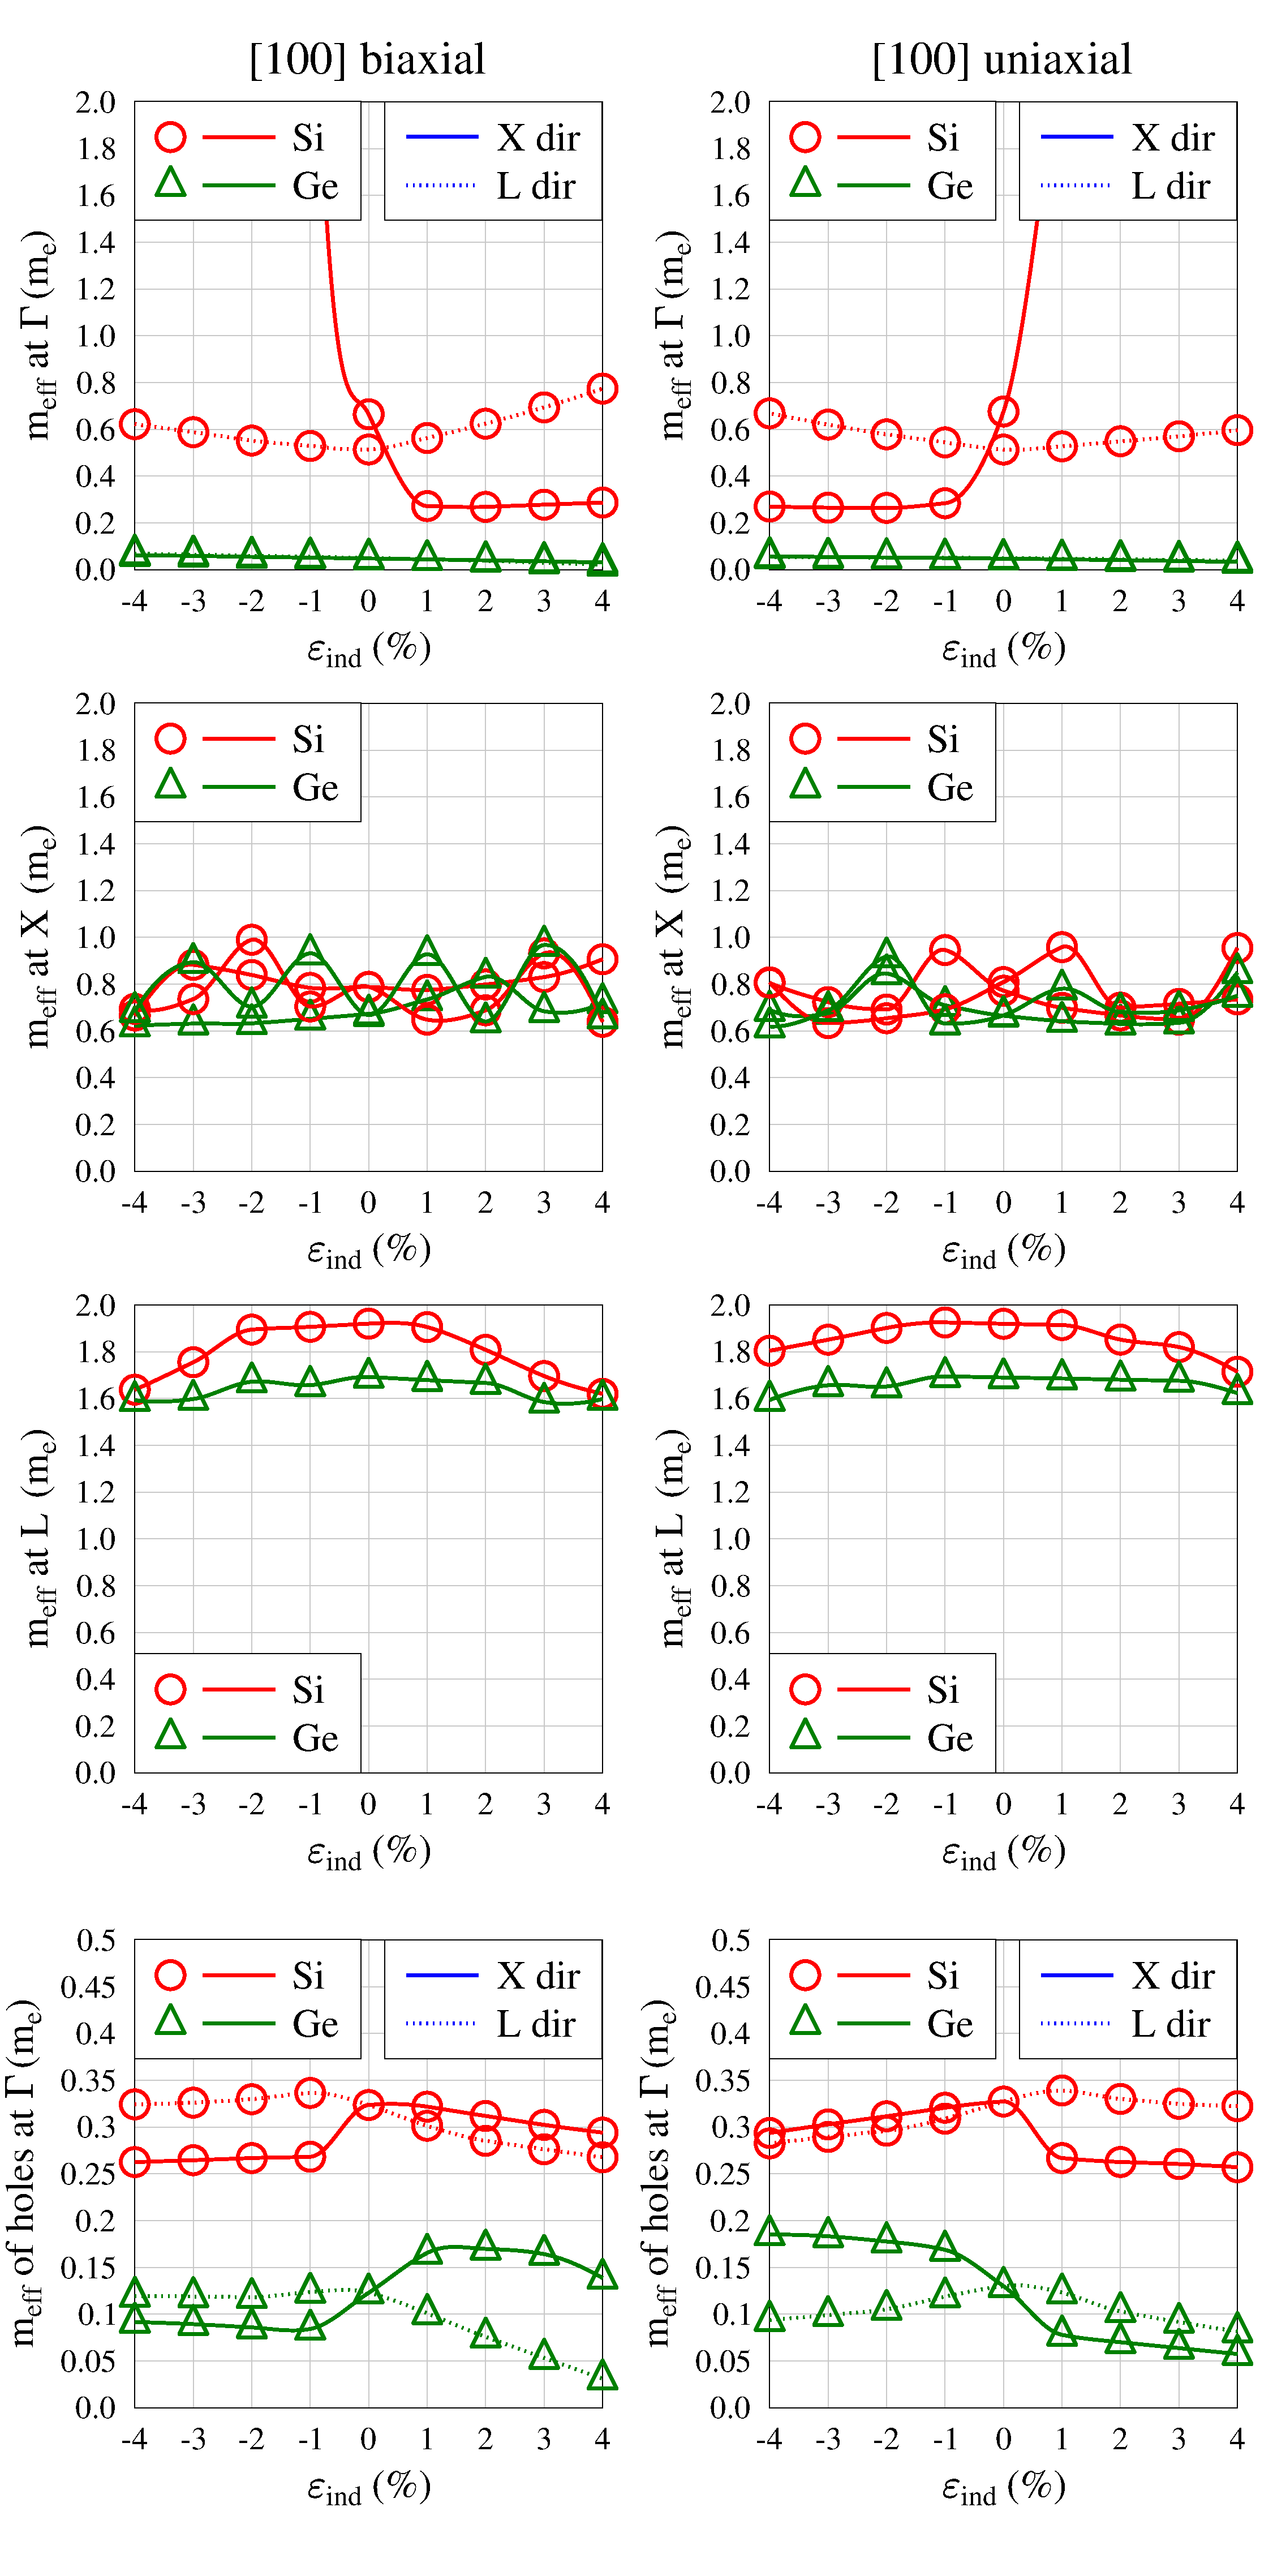
\includegraphics[width=0.7\textwidth]{strain/mass_100.pdf}
    \caption{Effective masses dependent on strains with respect to ${[100]}$ axis; red circles - Si, green triangles - Ge; at $\Gamma$: solid line - $\Gamma$-$X$ direction, dotted line - $\Gamma$-$X$ direction.} 
    \label{Fig:strain_mass_100}
\end{figure}

\begin{figure}[!htbp]
    \centering
    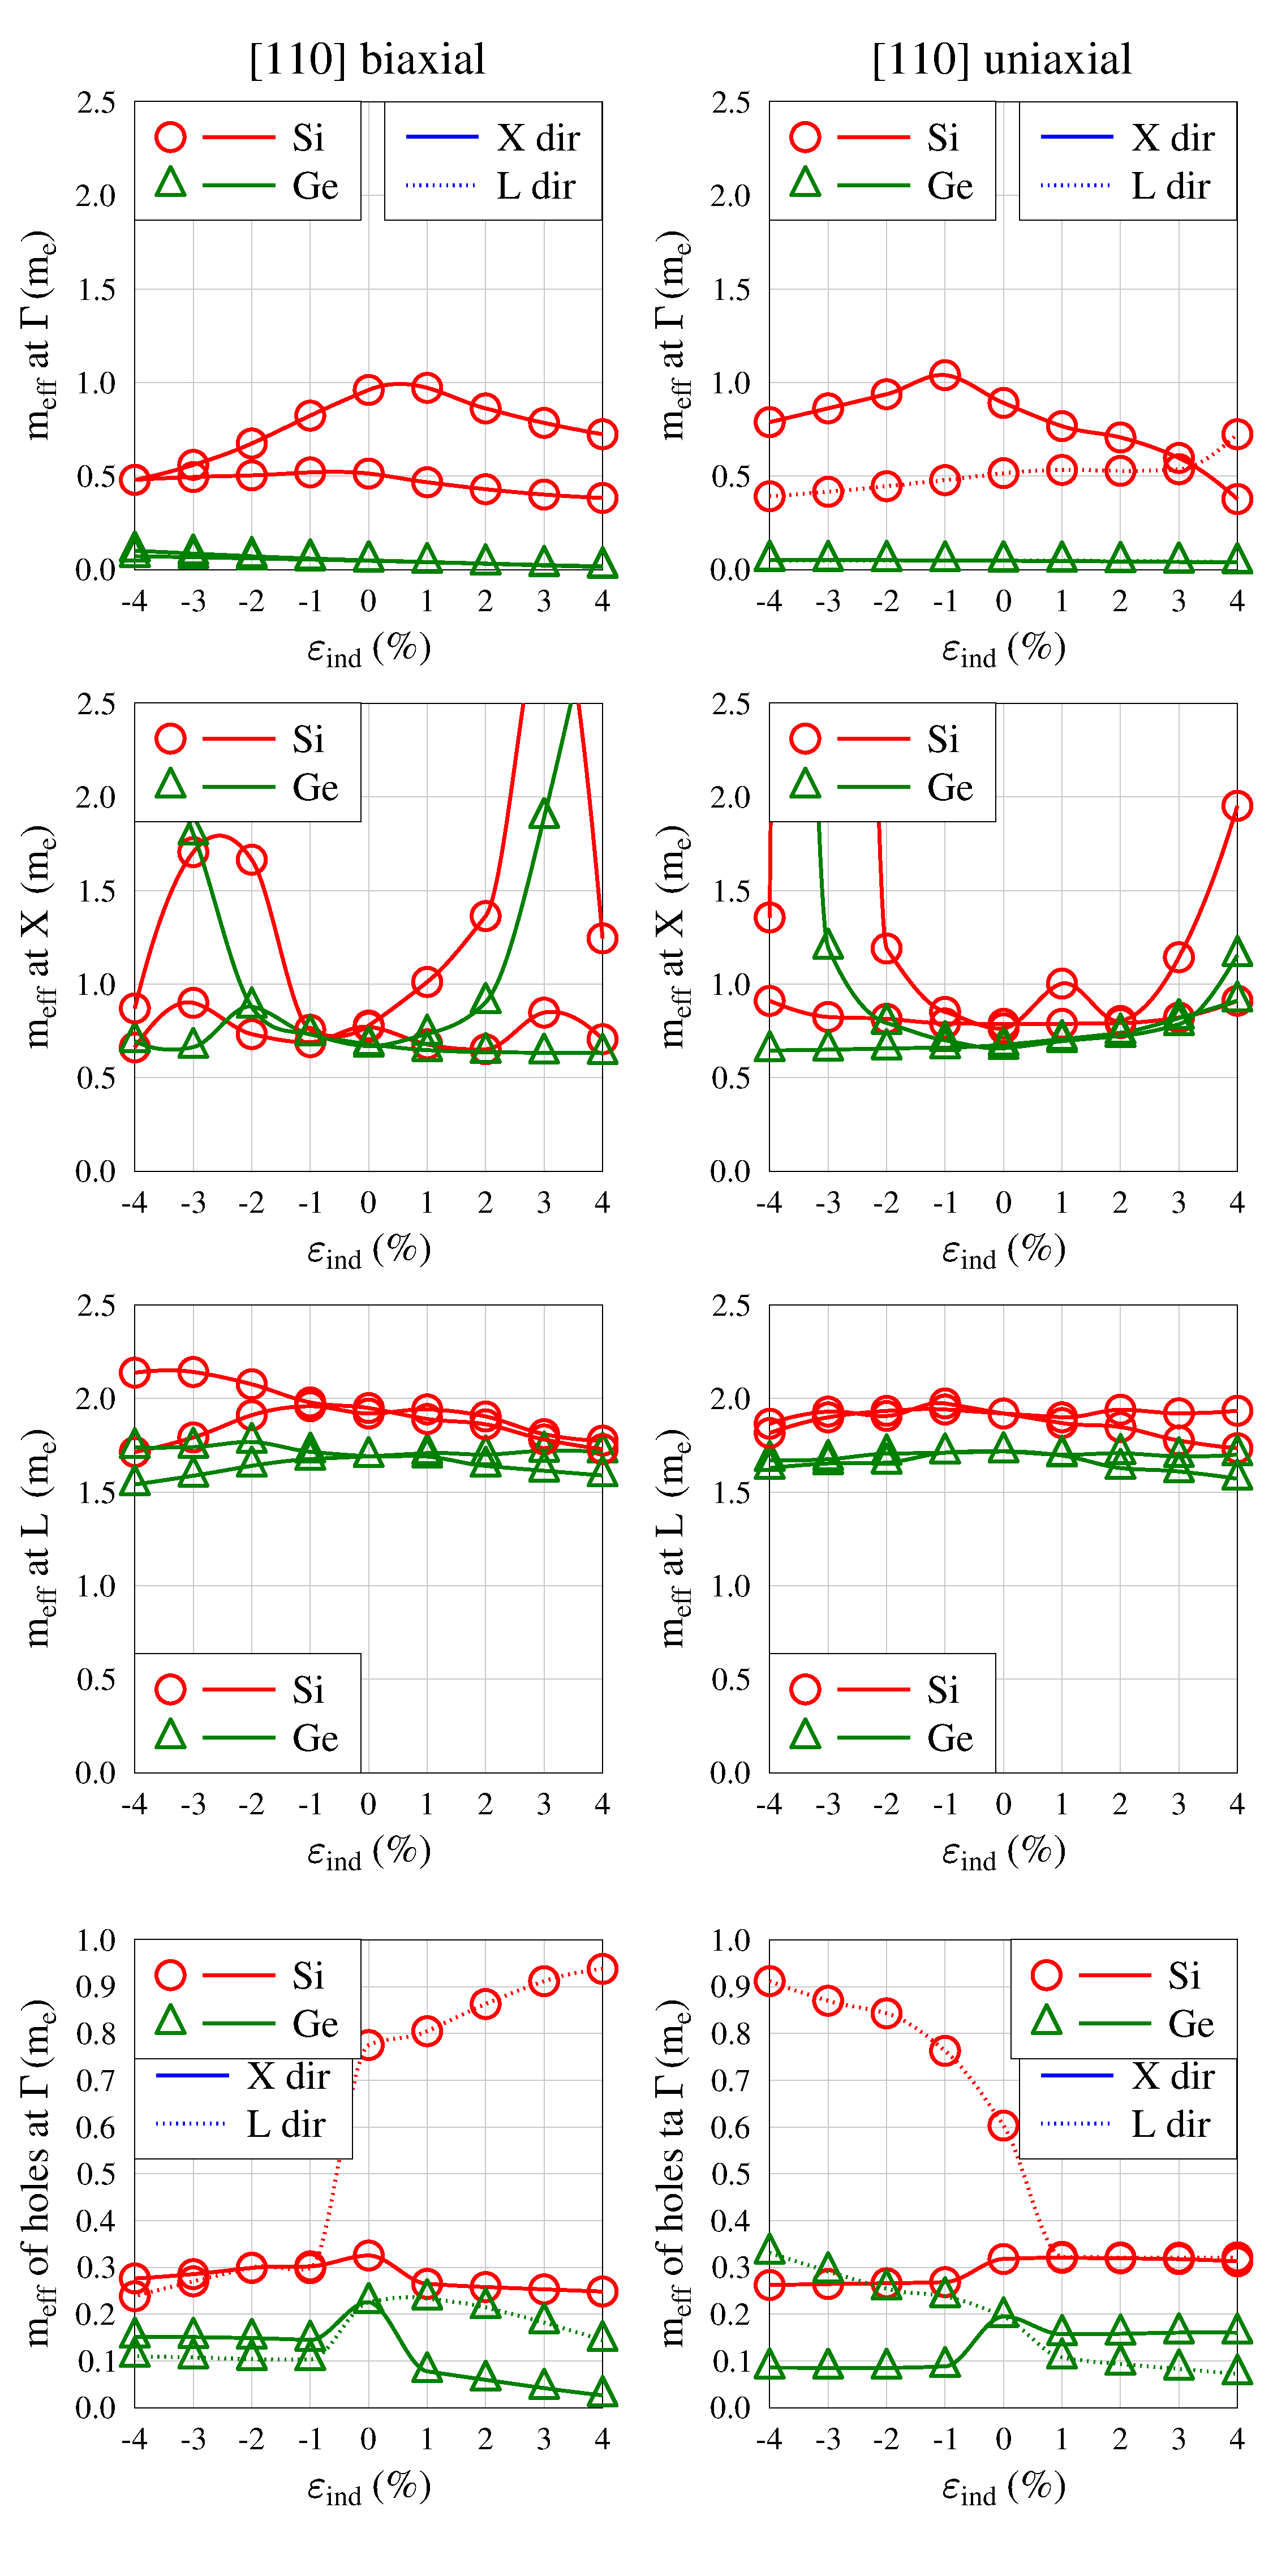
\includegraphics[width=0.7\textwidth]{strain/mass_110.pdf}
    \caption{Effective masses dependent on strains with respect to ${[110]}$ axis; red circles - Si, green triangles - Ge; at $\Gamma$: solid line - $\Gamma$-$X$ direction, dotted line - $\Gamma$-$X$ direction.} 
    \label{Fig:strain_mass_110}
\end{figure}

\begin{figure}[!htbp]
    \centering
    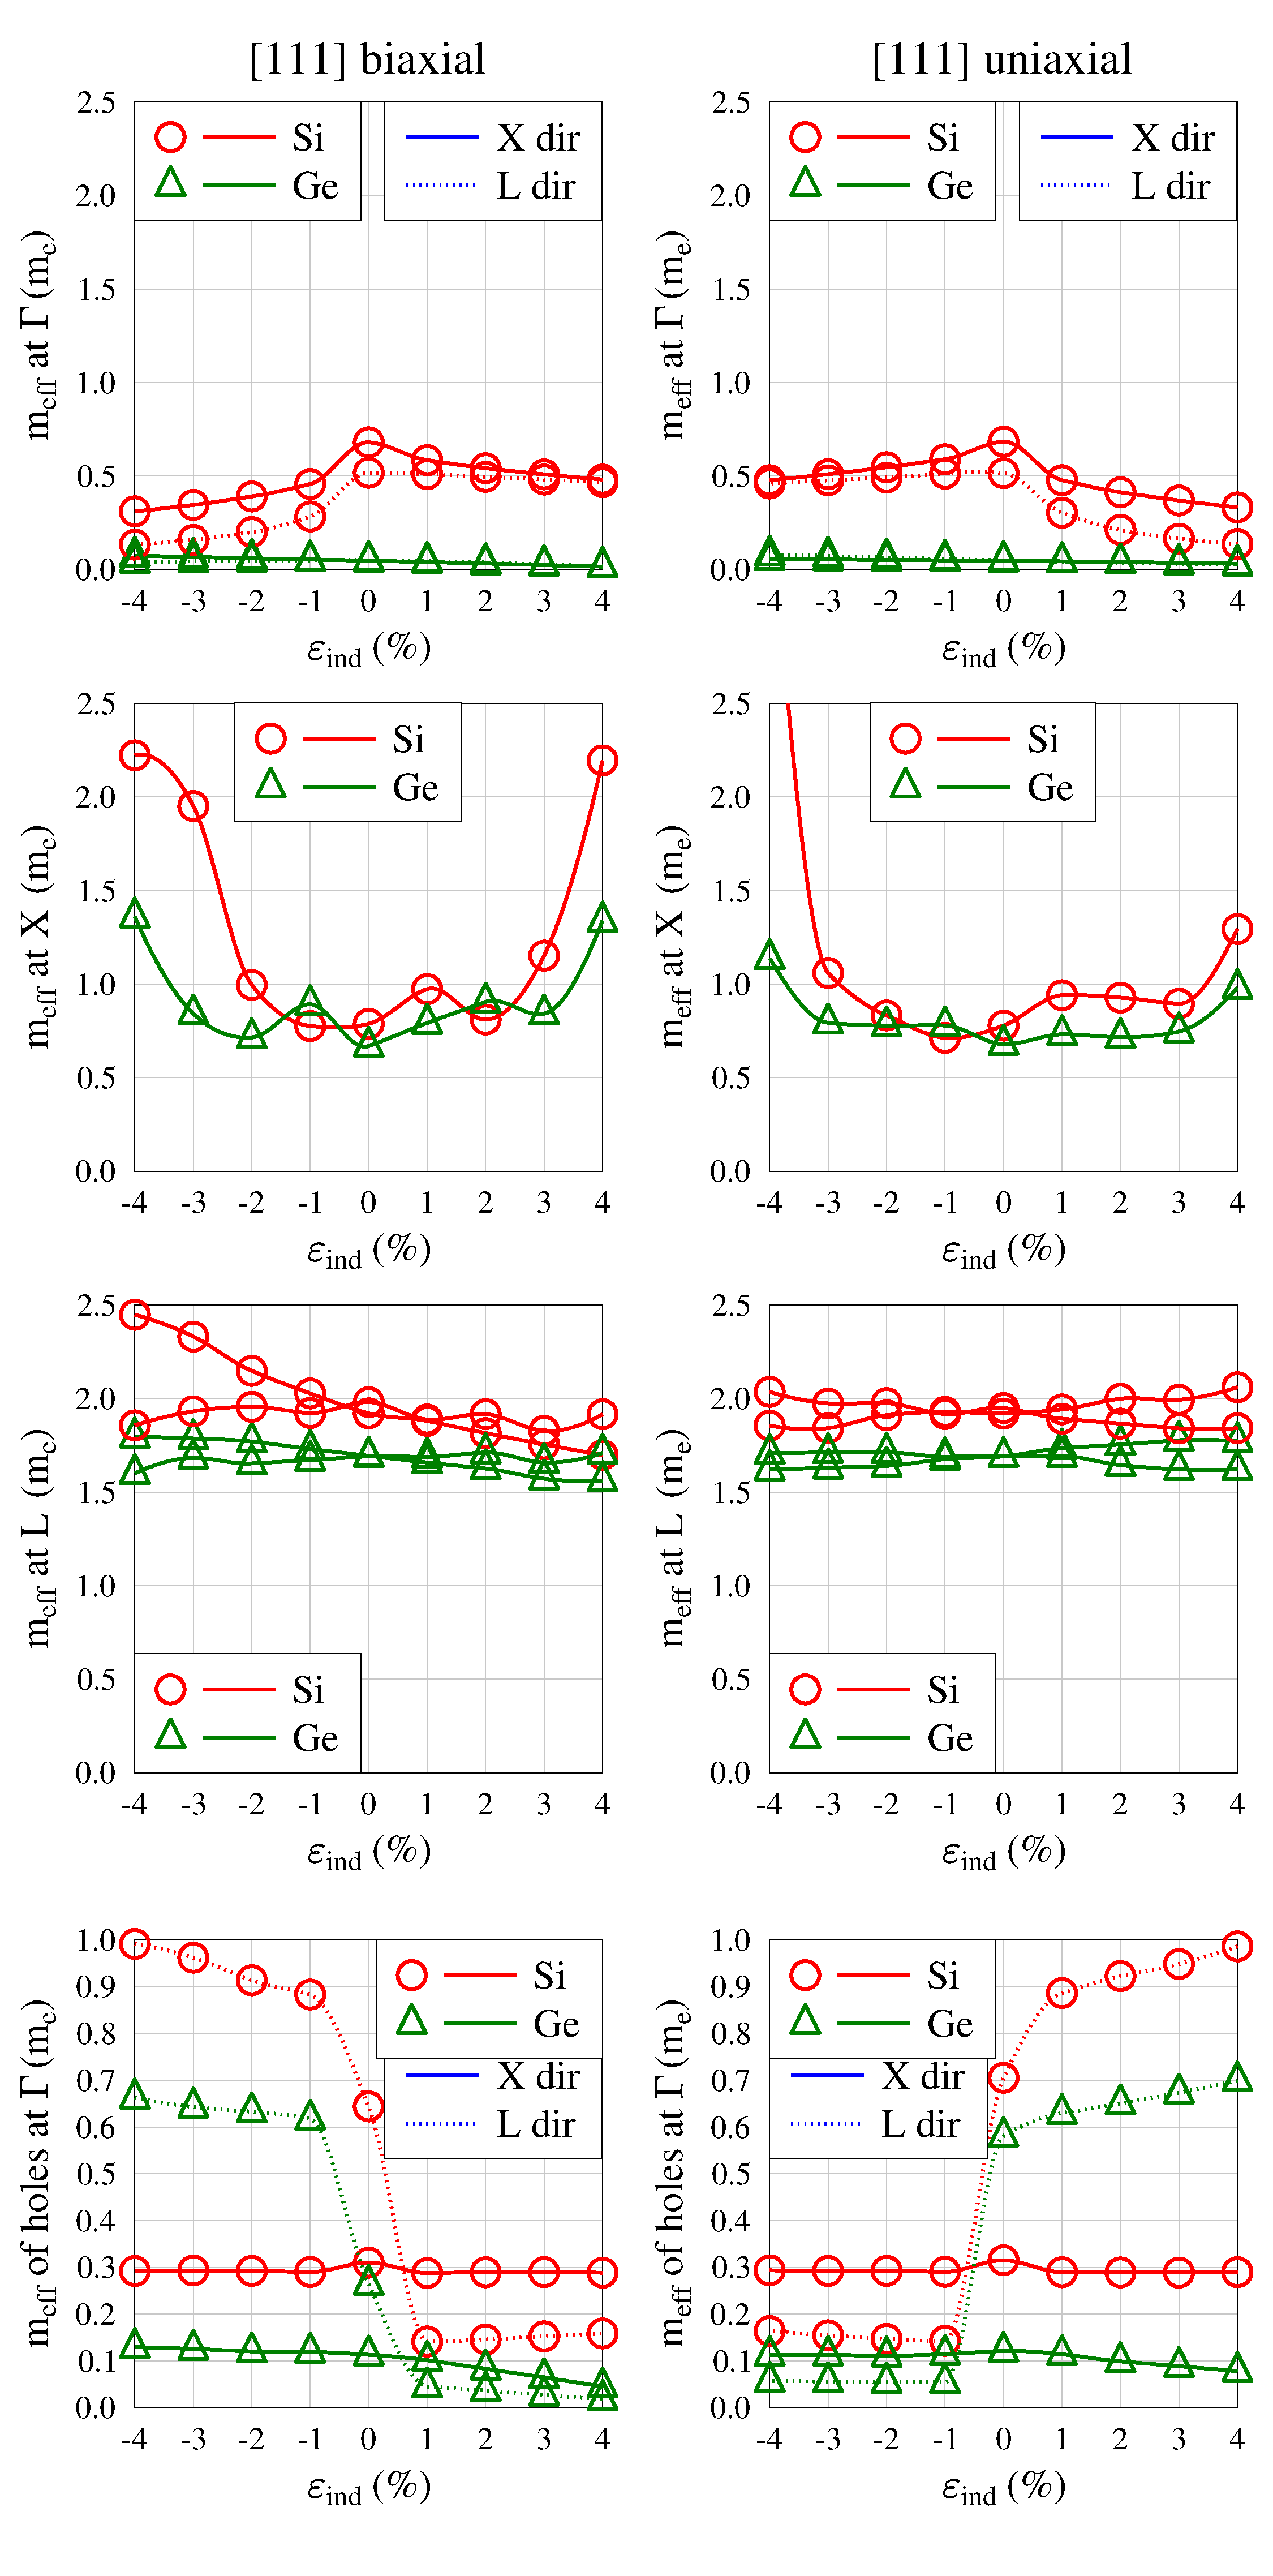
\includegraphics[width=0.7\textwidth]{strain/mass_111.pdf}
    \caption{Effective masses dependent on strains with respect to ${[111]}$ axis; red circles - Si, green triangles - Ge; at $\Gamma$: solid line - $\Gamma$-$X$ direction, dotted line - $\Gamma$-$X$ direction.} 
    \label{Fig:strain_mass_111}
\end{figure}

\begin{figure}[!htbp]
    \centering
    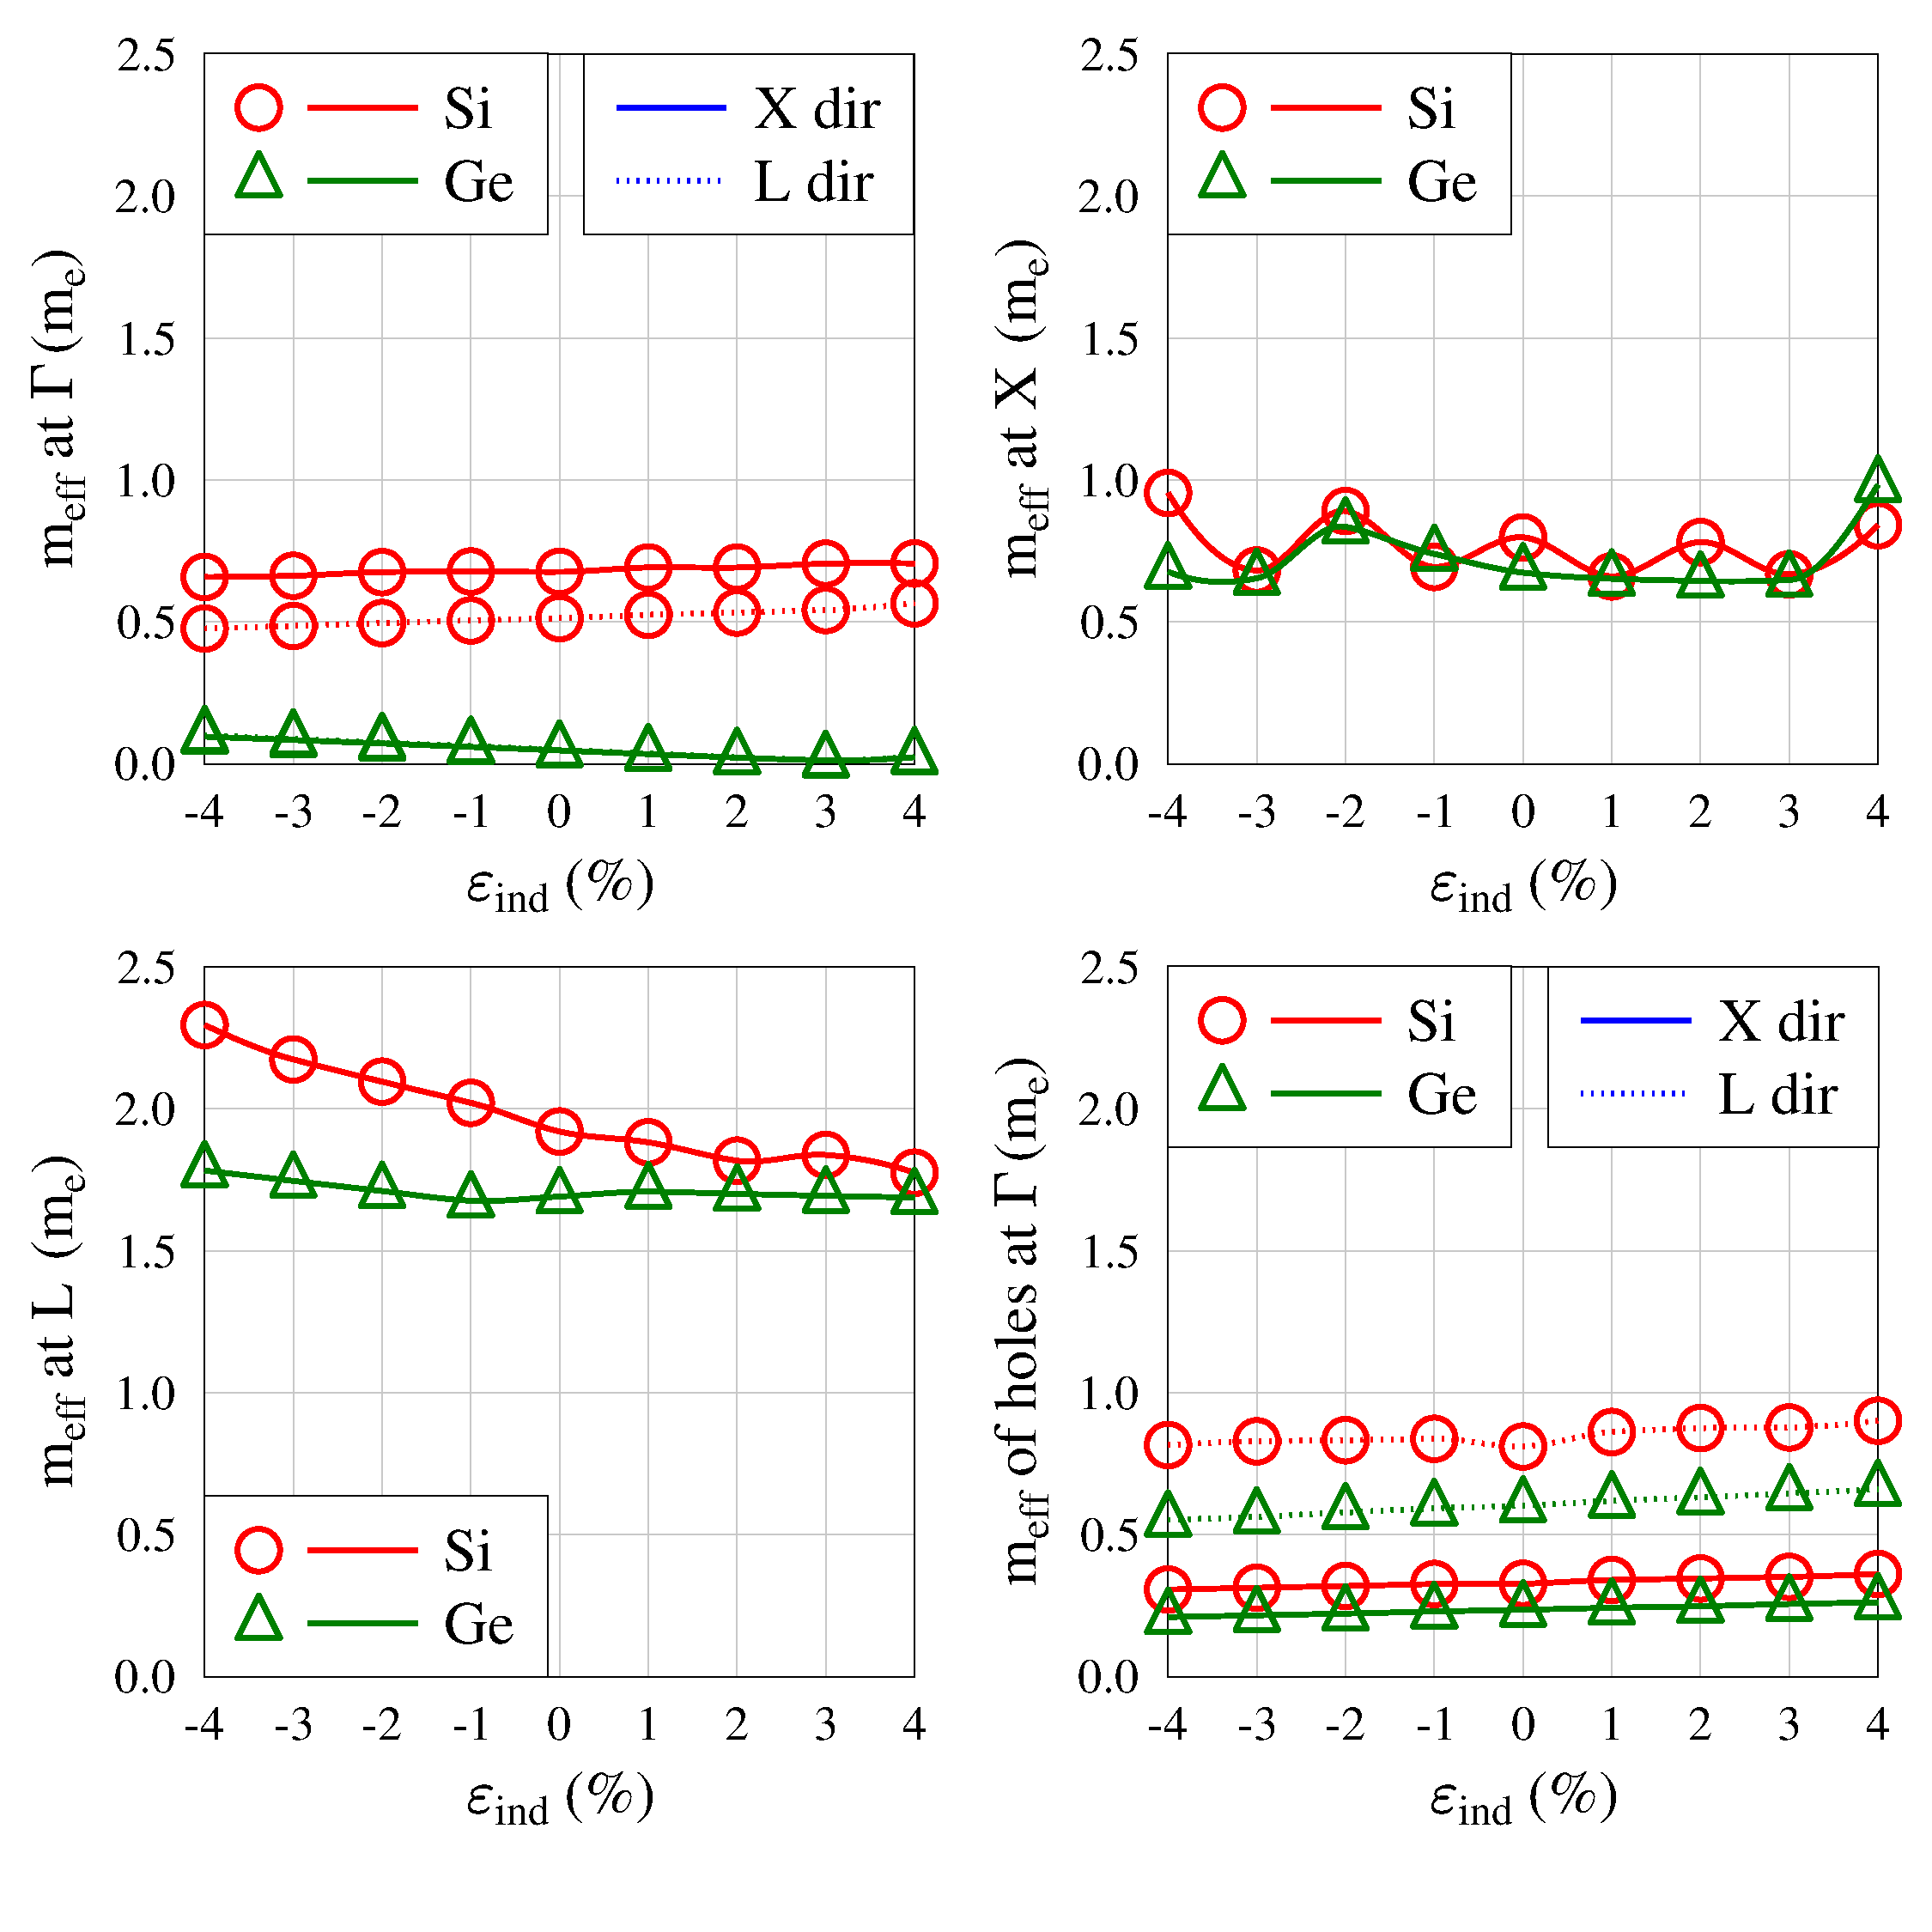
\includegraphics[width=0.7\textwidth]{strain/mass_iso.pdf}
    \caption{Effective masses dependent on isotropic strains; red circles - Si, green triangles - Ge; at $\Gamma$: solid line - $\Gamma$-$X$ direction, dotted line - $\Gamma$-$X$ direction.} 
    \label{Fig:strain_mass_iso}
\end{figure}
\newpage
\ornament

\section{Charge carriers mobility}

In addition to calculation of effective masses, the effect of strain on carrier mobility has been estimated.
The mobility is related to effective mass by scattering time, as follows
\begin{equation}
    \label{Eq:strain_mobility}
    \mu=\frac{q}{m^*}\bar{\tau},
\end{equation}
where $q$ is an elementary charge, and $\bar{\tau}$ is the average scattering time.
The scattering time, in general, depends on many factors connected with the scattering mechanisms which is not considered here.
Instead, an empirical model based on Monte Carlo simulations was used to evaluate the average scattering time for electrons \cite{scattering-time}:

\begin{equation}
\begin{split}
    \bar{\tau}_n =& \tau_0 + \tau_1 \cdot exp\Bigg(C_1 \cdot \bigg(\frac{T_n}{300 K}+C_0\bigg)^2 + \\
   & + C_2 \cdot \bigg(\frac{T_n}{300 K}+C_0\bigg) + C_3 \cdot \bigg(\frac{T_L}{300 K}\bigg) \Bigg) \\
\end{split}
\label{Eq:strain_time}
\end{equation}

where $T_n$ is the electron temperature, $T_L$ is the lattice temperature, while all of the $\tau$ and $C$ are material dependent constants (shown in Tab. \ref{Tab:strain_time}).
Formula \ref{Eq:strain_time} has been used here for calculating scattering time of electrons.
In the case of holes the scattering time is independent of carrier and lattice temperatures:
\begin{equation}
\label{Eq:strain_holes_time}
\bar{\tau}_p =\tau_2.
\end{equation}

\begin{table}[!htbp]
\centering
\caption{Material parameters for average scattering time  ( Eq. \ref{Eq:strain_time}) \cite{scattering-time}. $\tau$ are given in (ps).}
\begin{tabular}{|c|c|c|c|c|c|c|c|}
\hline
 & $\tau_0$ & $\tau_1$ & $C_0$ & $C_1$  & $C_2$ & $C_3$ & $\tau_2$ \\ \hline
Si       & 1             & -0.538        & 0     & 0.0015 & -0.09 & 0.17  & 0.4           \\ \hline
Ge       & 0.26          & 1.49          & 0     & -0.434 & 1.322 & 0     & 0.4           \\ \hline
\end{tabular}
\label{Tab:strain_time}
\end{table}

For given temperatures, the mobility changes are completely established by effective mass (Eq. \ref{Eq:strain_time}).
For unstrained materials the mobilities for both electrons and holes are known.
For Si it is $\leq 1400 \frac{cm^2}{V\cdot s}$ and $\leq 450 \frac{cm^2}{V\cdot s}$ for electrons and holes respectively, and for Ge similarly $\leq 3900 \frac{cm^2}{V\cdot s}$ and $\leq 1900 \frac{cm^2}{V\cdot s}$ (according to NSM Archive \cite{nsm}).
If we assume that the strain does not affect the scattering time, the strain dependent mobilities can be evaluated.
Examples of such calculations are presented in Fig. \ref{Fig:strain_mobility}.
First of all one can see that presented results agree well with tabular data at equilibrium state.
It can be also observed that the strain induced changes in effective masses affect significantly the mobilities.
In extreme cases they can change even by an order of magnitude.
 
 \begin{figure}[!htbp]
    \centering
    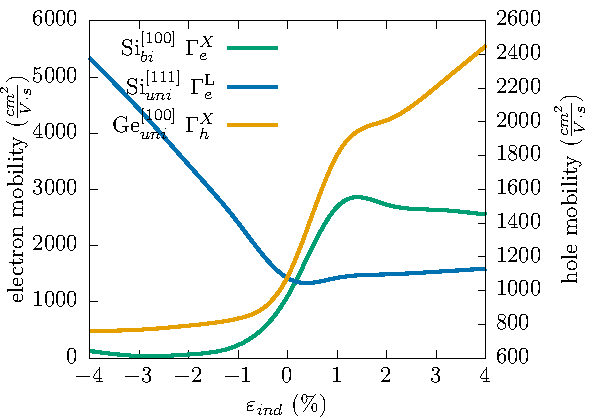
\includegraphics[width=0.7\textwidth]{strain/mobility.pdf}
    \caption{Carrier mobility examples calculated for $T_n,\,T_L=300 K$.} 
    \label{Fig:strain_mobility}
\end{figure}

\ornament

\section{Precision and accuracy of the results}

When \DFT\ results are presented the question about their precision and accuracy always arises.
The term ''precision'' in this context refers to the accuracy of calculations at given methods used within \DFT, i.e. their deviation from the exact result if it existed.
Since the ''exact'' result does not exist, the only way of estimating the precision is to compare the results with analogous ones, given by other codes, among which the full potential implementations seem to be most credible.
This issue is widely discussed in \cite{accuracy} where a special parameter $\Delta$ is introduced as a measure of discrepancy between \EOS\ for a sample of crystals calculated by a given pair of codes.
This parameter, when used in reference to full potential codes becomes a measure of precision.
In turn, the term ''accuracy'' refers to the agreement of computational results with experimental data, and it seems that an ultimate criterion to value various \DFT\ methods/codes is to compare the results with the experiment.
In the light of these remarks the discuss of the results presented is conducted below. 

The table in Fig.4 in \cite{offsets-Kresse} shows a comparisons of $\Delta$ parameter for most known \DFT\ methods, in reference to full-potential methods.
The PAW JTH/ABINIT, used in this work (in even newer version than in \cite{offsets-Kresse}), has there a very good ($0.6$) value.
Only VASP and various full potential codes show slightly better values (the lowest average value is $0.5$ and the highest is $13.3$).
In results presented here, this kind of \PAW\ datasets has been used in all the structural calculations and in the case of deformation potentials as well.
Taking into account that the rigorous convergence tests have been performed, the precision of presented results should be high.
Regarding the accuracy, it is also very satisfactory, as shows the comparison with the available experimental data.
E.g. the Tab. \ref{Tab:strain_lattice} shows an excellent agreement of the calculated lattice constants with experimental ones.
Also the elastic constants, although defined here in an unconventional way, when transformed to the standard ones agree well with the textbook data (see Tab. \ref{Tab:strain_elastic}).

\begin{figure}
    \centering
    \includegraphics[width=0.7\textwidth]{/strain/vs.pdf}
    \caption{Comparison between Wien2k (red line) and ABINIT with \mBJLDA\ (blue line) band structure of Ge in equilibrium state.} 
    \label{Fig:strain_wien-abinit}
\end{figure}

The calculations of band energies, gaps and effective masses have been performed using different method (\HGH\ joined with the \mBJLDA\ XC potential, see Sect. \ref{chap:methods}), and thus require a separate discussion of precision and accuracy.
As described in Sect. \ref{chap:methods}, the \mBJLDA\ cTB$09$ parameter (called here \textit{c}) has been fitted to get correct (experimental band gaps) and specially treated for strained systems (Eq. \ref{Eq:ctbo9}).
Figure \ref{Fig:strain_wien-abinit} shows a comparison of Ge band structure obtained in this work and by Wien2k code.
And one can see that the agreement is very good.
This means that conducted calculations are expected to be highly precise.
As far as the accuracy is concerned the agreement with the available experimental data shown in Fig. \ref{Fig:strain_exp} is very good. 

The accuracy of effective masses is an important issue to comment, since this is a known fact that the \mBJLDA\ functional overestimates effective masses by $20-30\%$ \cite{mbjlda_precision}, which is then a systematic error.
Surprisingly, the approach used in this work does not quite reflect this tendency.
As Tab. \ref{Tab:strain_masses} shows, the effective masses calculated here (in a very strict mathematical approach) sometimes are even lower than the experimental ones, but the overall agreement is quite satisfactory.
Nevertheless, the results presented here can certainly be regarded as a good qualitative picture (with rather low quantitative uncertainty) of masses vs. strains variation.

The calculations of the deformation potentials, particularly those describing the absolute changes in energies, are a delicate issue.
For the top of \VB, they have been done with the use of \PAW\ atomic datasets.
The same which gave very satisfactory structural parameters.
Here, the \DFT\ band gap problem does not exist since we consider only the \VB\ top energy with respect to the unified energy reference point.
Thus, the discrepancy of provided results with the literature data is surprising.
For this reason there have been included a precise description of the method used (see Chap. \ref{chap:methods}), so that the reproduction of the data or questioning the approach would be possible.

\ornament